\documentclass[12pt]{scrartcl}
\input{NiaLatexHelpers/nia_defs.tex}

\title{\vspace{-2em} Boolean Problems and CodingBat}
\author{}
\date{}

\newcommand{\pyTrue}[1][]{\pythonl[fontsize=#1]{True}\xspace}
\newcommand{\pyFalse}[1][]{\pythonl[fontsize=#1]{False}\xspace}

\begin{document}
\maketitle

\vspace{-6em}
\section{Turning a Word Problem Into Code}
Consider the following silly problem:
\begin{callout}
    A pair of beavers can build a dam if the river is flowing slowly and they have wood. Let \pythonl{fastRiver} be a \pyTrue or \pyFalse variable (which is called a \pythonl{bool}) that is true if the river is flowing fast. Let \pythonl{hasWood} represent whether the beavers have wood. Write a function \pythonl{canBuildDam(fastRiver, hasWood)} that returns (aka outputs) \pyTrue if the beavers can build their dam.
\end{callout}
Reading this problem, we can recognize that we're using \pyTrue or \pyFalse to represent certain real world properties. \pythonl{fastRiver} is \pyTrue if the river is moving fast, so if the river is moving slow (aka not fast), \pythonl{fastRiver} would be false. Similarly, if the beavers have wood, \pythonl{hasWood} would be \pyTrue, while if the beavers don't have wood, \pythonl{hasWood} would be false.

\medskip
\vspace{1em}

\begin{figure}[H]
    \begin{minipage}{0.48\textwidth}
        \centering
        \small
        \begin{tabular}{l|l}
        \pythonl[fontsize=\small]{fastRiver} &  Meaning\\
            \hline
        \pyTrue[\small] & River is moving fast.\\
        \pyFalse[\small] & River is moving slow.
        \end{tabular}
    \end{minipage}
    \hfill
    \begin{minipage}{0.48\textwidth}
        \centering
        \small
        \begin{tabular}{l|l}
       \pythonl[fontsize=\small]{hasWood} &  Meaning\\
            \hline
        \pyTrue[\small] & The beavers have wood.\\
        \pyFalse[\small] & The beavers have no wood.
        \end{tabular}
    \end{minipage}

    \medskip

    \caption*{Bools and What They Mean}
\end{figure}

Okay, so we know what the variables represent, but what would the function look like? Well, we know that we're trying to return \pyTrue if the beavers can build their dam. And the beavers can only build their dam if the river is moving slow (so \pythonl{fastRiver} must be false) and when they have wood (so \pythonl{hasWood} is true). So if \pythonl{not fastRiver} and the beavers \pythonl{hasWood}, the beavers can buld the dam. So the function would be:

\newpage
\begin{python}
def canBuildDam(fastRiver, hasWood):
    if (not fastRiver) and hasWood:
        return True
    else:
        return False
\end{python}

And viola! Our first boolean problem is solved. By boolean problem, what I mean is we wrote a function that takes in only \pyTrue or \pyFalse variables known as \pythonl{bool}s, and then the function outputs \pyTrue or \pyFalse (aka a \pythonl{bool}).

Problems involving \pyTrue and \pyFalse come up so much in programming as we use \pythonl{bool}s for decision making in programs. Think of your own life and how you map out your day. You may make a mental list in your head like the following.
\begin{center}
    \small
    Plan for a Birthday Party
    \begin{enumerate}
        \item Check if we're out of any cake ingredients.
        \item If out of milk, head to grocery store.
        \item Check if any streamers from last year are in the basement.
        \item If not, go to the party store.
    \end{enumerate}
\end{center}
This To-Do list is using booleans! If \pythonl{outOfMilk} is \pyTrue, then we need to go to the grocery store to buy milk. If \pythonl{hasStreamers} is \pyFalse, then we need to buy some more at the party store. \pyTrue and \pyFalse are a way to let decision-making be very precise, allowing us to tell computers, which are very rigid, to do exactly what we want. Mastering using booleans will serve you well as a programmer.

\newpage
\section{Using Tables to Solve Boolean Problems}
Consider another silly problem:
\begin{callout}
    A couple is taking a stroll at a park. Write a function \pythonl{isDry(raining, haveUmbrella)} that represents whether the couple will stay dry or not.
\end{callout}
This time, this problem description didn't tell us what \pythonl{raining} and \pythonl{haveUmbrella} represent. Often coding problems won't give us all the details we would like. But the names of these variables make their meanings clear: \pythonl{raining} is \pyTrue if it is raining, and \pythonl{haveUmbrella} is \pyTrue if the couple has an umbrella.

\medskip
\vspace{1em}

\begin{figure}[H]
    \centering
    \begin{tabular}{p{2.5cm}|p{5cm}}
        \pythonl{raining} & Meaning \\
        \hline
        \pyTrue & It is raining. \\
        \pyFalse & It's not raining.
    \end{tabular}
    
    \vspace{2em}
    
    \begin{tabular}{p{2.5cm}|p{5cm}}
        \pythonl{haveUmbrella} & Meaning \\
        \hline
        \pyTrue & The couple has an umbrella. \\
        \pyFalse & The couple does not have an umbrella.
    \end{tabular}

    \vspace{1em}

    \caption*{More Variable Meanings}
\end{figure}

It's not that obvious when \pythonl{isDry} should return \pyTrue. We'll have to think logically. If it's not raining---that is, if \pythonl{raining} is \pyFalse---then we should return \pyTrue always, as the couple won't get wet without rain. If it is raining, the couple will still not get wet if they have an umbrella. How could we represent these relationships? By a table!

\begin{figure}[H]
    \centering
    \begin{tabular}{cc|c|c|}
        & \hidevline{} & \multicolumn{2}{c}{\pythonl{haveUmbrella}} \\ 
        &  \hidevline{} & \hidevline{\pyTrue} & \hidevline{\pyFalse} \\
        \cline{3-4}
        \multirow{2}{*}{\pythonl{raining}} & \pyTrue & Dry! & Wet. \\
        \cline{3-4}
        & \pyFalse & Dry! & Dry! \\
        \cline{3-4}
    \end{tabular}
    \medskip
    \caption*{Converted to True and False}
\end{figure}

So it looks like the only scenario where we're wet is if it is raining and we have no umbrella. Since we return \pyTrue when we are dry, and \pyFalse when we are wet, we can rewrite the table as follows:

\begin{figure}[H]
    \centering
    \begin{tabular}{cc|c|c|}
        & \hidevline{} & \multicolumn{2}{c}{\pythonl{haveUmbrella}} \\ 
        &  \hidevline{} & \hidevline{\pyTrue} & \hidevline{\pyFalse} \\
        \cline{3-4}
        \multirow{2}{*}{\pythonl{raining}} & \pyTrue & \pyTrue & \pyFalse \\
        \cline{3-4}
        & \pyFalse & \pyTrue & \pyTrue \\
        \cline{3-4}
    \end{tabular}
    \medskip
    \caption*{How the Input Affects the Result}
\end{figure}

So if it's \pythonl{not raining} or they \pythonl{haveUmbrella}, then the couple is dry, which is a \pythonl{True}. Therefore, our function would be:

\begin{python}
    def isDry(raining, haveUmbrella):
        if (not raining) or haveUmbrella:
            return True
        else:
            return False
\end{python}

\bigskip 

So to summarize our method for boolean problems:

\begin{callout}
    \textbf{\large How to Write Boolean Functions:}
    \begin{itemize}
        \item Determine what the input variables mean in English when they are \pyTrue or \pyFalse. A chart is handy here.
        \item Create a table that shows the result depending on the input.
        \item Determine when we return \pyTrue and \pyFalse based on the result. What does an output of \pyTrue mean in the conext of the problem?
        \item If you need help with figuring out when to return \pyTrue and \pyFalse, see the next section!
    \end{itemize}
\end{callout}

\section{Figuring Out When to Return True and False}
In the previous examples, we intuited when to return True and False. We recognized that the beavers need wood and a slow river to build a dam, so \pythonl{(not fastRiver) and hasWood} was our if statement. Similarly, we recognized that for the couple to stay wet, either it needed to not rain or they needed an umbrella, so our if statement was \pythonl{(not raining) or haveUmbrella}. But what about if you're not sure when to return True? Maybe you're struggling to intuit it. Here's a helpful method:

Remember that there were four possiblities for input and output in the beaver problem:

\begin{figure}[H]
    \centering
    \begin{tabular}{cc|c|c|}
        & \hidevline{} & \multicolumn{2}{c}{\pythonl{hasWood}} \\ 
        &  \hidevline{} & \hidevline{\pyTrue} & \hidevline{\pyFalse} \\
        \cline{3-4}
        \multirow{2}{*}{\pythonl{fastRiver}} & \pyTrue & \pyFalse & \pyFalse \\
        \cline{3-4}
        & \pyFalse & \pyTrue & \pyFalse \\
        \cline{3-4}
    \end{tabular}
    \medskip
    \caption*{The Square For The Beaver Problem}
\end{figure}

Well, we can write every single scenario and return \pyTrue or \pyFalse for each!

\maynewpage
\begin{python}
def canBuildDam(fastRiver, hasWood):
    if not fastRiver and not hasWood:
        return False
    if not fastRiver and hasWood:
        return True
    if fastRiver and not hasWood:
        return False
    if fastRiver and hasWood:
        return False
\end{python}
And we're done! This is also a perfectly valid solution. If you want, you can recognize that we could just combine all the false's together into one else, creating:
\begin{python}
    def canBuildDam(fastRiver, hasWood):
        if not fastRiver and hasWood:
            return True
        else:
            return False
\end{python}
which is what we had before. So even if you can't intuit the logic in your head, you can always write a brute-force answer by hadnling every possibilitiy. Your code won't always be the most efficient, but we can care about efficiency later.

\section{The Nitty-Gritty: What does \texorpdfstring{\pythonl{not}, \pythonl{or}, and \pythonl{and} do?}{NOT, OR, and AND do?}}

When we write ``\pythonl{if (not raining) or haveUmbrella}'', what does \pythonl{or} and \pythonl{not} actually tell the computer? We understand \pythonl{if} as allowing us to do code only some of the time. How about \pythonl{and}, \pythonl{or} and \pythonl{not}? Is there a good understanding of them?

\subsection*{\texorpdfstring{\pythonl{not}}{NOT} Meaning}
To the computer, \pythonl{not} flips a \pyTrue to a \pyFalse and vice versa.
\begin{figure}[H]
    \centering
\begin{tabular}{c|c}
    \pythonl{raining} & \pythonl{not raining} \\
    \hline
    \pyTrue & \pyFalse \\
    \pyFalse & \pyTrue
\end{tabular}
\end{figure}

So if we want code to run only if something is not the case, we can use \pythonl{not}!

\subsection*{\texorpdfstring{\pythonl{and}}{AND} Meaning}

The keyword \pythonl{and} lets us combine two variables and only output \pyTrue if both input variables are \pyTrue.

\begin{figure}[H]
    \centering
\begin{tabular}{cc|c}
    \pythonl{happy} & \pythonl{noHomework} & \pythonl{happy and noHomework}\\
    \hline
    \pyFalse & \pyFalse & \pyFalse \\
    \pyFalse & \pyTrue & \pyFalse \\
    \pyTrue & \pyFalse & \pyFalse \\
    \pyTrue & \pyTrue & \pyTrue
\end{tabular}
\end{figure}
This chart (and the one for \pythonl{not} is called a \textit{Truth Table}, as it shows how inputs correspond to outputs. Notice we consider all possibilities: both inputs are false, one is true and one is false, and both are true. These are four possibilities, and the reason there is four is because
\[2 \text{ possibilities for one variable} \times 2 \text{ possibilities for another} = 4 \text{ possibilities}\]
The keyword \pythonl{and} only outputs true if both inputs are true. Notice also that this chart could also be represented as a square like we did before with the \pythonl{isDry} problem:

\begin{figure}[H]
    \centering
    \begin{tabular}{cc|c|c|}
        & \hidevline{} & \multicolumn{2}{c}{\pythonl{noHomework}} \\ 
        &  \hidevline{} & \hidevline{\pyTrue} & \hidevline{\pyFalse} \\
        \cline{3-4}
        \multirow{2}{*}{\pythonl{happy}} & \pyTrue & \pyTrue & \pyFalse \\
        \cline{3-4}
        & \pyFalse & \pyFalse] & \pyFalse \\
        \cline{3-4}
    \end{tabular}
    \medskip
    \caption*{Result of \pythonl{happy and noHomework}}
\end{figure}


\subsection*{\texorpdfstring{\pythonl{or}}{OR} Meaning}

The keyword \pythonl{or} lets us combine two variables and output \pyTrue if at least one variable is \pyTrue. Here is an example truth table:

\begin{figure}[H]
    \centering
\begin{tabular}{cc|c}
    \pythonl{haveCoke} & \pythonl{havePepsi} & \pythonl{haveCoke or havePepsi}\\
    \hline
    \pyFalse & \pyFalse & \pyFalse \\
    \pyFalse & \pyTrue & \pyTrue \\
    \pyTrue & \pyFalse & \pyTrue \\
    \pyTrue & \pyTrue & \pyTrue
\end{tabular}
\end{figure}

Once again we have $2 \times 2 = 4$ possibilities for the input, so there's four rows in our chart. Once again, we could represent this chart as a square:

\begin{figure}[H]
    \centering
    \begin{tabular}{cc|c|c|}
        & \hidevline{} & \multicolumn{2}{c}{\pythonl{havePepsi}} \\ 
        &  \hidevline{} & \hidevline{\pyTrue} & \hidevline{\pyFalse} \\
        \cline{3-4}
        \multirow{2}{*}{\pythonl{haveCoke}} & \pyTrue & \pyTrue & \pyTrue \\
        \cline{3-4}
        & \pyFalse & \pyTrue & \pyFalse \\
        \cline{3-4}
    \end{tabular}
    \medskip
    \caption*{Result of \pythonl{haveCoke or havePepsi}}
\end{figure}

There is something interesting here about \pythonl{or} in programming. In English, we may use the word ``or'' in a few different ways:
\begin{itemize}
    \item ``Can you hang out today \textit{or} tonight?''
    \item ``Would you like the pasta \textit{or} the burrito for your meal?''
    \item ``Would you like sugar \textit{or} cream in your coffee?''
\end{itemize}
In response to the first question, you may answer ``Yes, I can hang out today or tonight.'' What you mean is that either time works, and potentially you could hang out for the day through the evening. The \pythonl{or} here is \textbf{inclusive}: Your friend answers yes (aka \pyTrue) to this question if today works, tonight works, or both works. 

Contrastly, question 2 expects \textit{either} ansewer but not both. You'll answer, ``I'd like the pasta,'' or you might answer, ``I'd like the burrito.'' It's unlikely you would answer, ``I'd like the pasta and the burrito,'' and that answer certainly isn't what waiter intended when asking the question. This is called an \textbf{exclusive} or.

The third quesiton is another inclusive or example. It's a perfectly valid response to reply, ``Yes, I would like sugar and cream in my coffee.'' You could also say, ``I want just sugar in my coffee'' or ``I just want cream in my coffee, no sugar.'' This \pythonl{or} here is inclusive: you are allowed to answer both.

The inclusive \pythonl{or} is what the keyword \pythonl{or} means in programming. There is a way to do exclusive or in Python, which has its own unique truth-table, but we'll talk about it another time.

\pythonl{not}, \pythonl{and}, or \pythonl{or} will be in the many if-statements you write as a programmer. Master these operators, and you can write powerful logic for all sorts of tasks. The reason we are focusing on boolean problems is partly to strengthen your skill in writing if-statements.

\section{Simplifying the Answer}

Let's revisit our \pythonl{canBuildDam} function:

\begin{python}
    def canBuildDam(fastRiver, hasWood):
        if (not fastRiver) and hasWood:
            return True
        else:
            return False
\end{python}

I want to remark that I put the parenthese around \pythonl{not fastRiver} for clarity purposes: They are not necessary in Python due to the order of operations, which we will talk about eventually. So the following code still works correctly:

\begin{python}
    def canBuildDam(fastRiver, hasWood):
        if not fastRiver and hasWood:
            return True
        else:
            return False
\end{python}

In the case where \pythonl{not fastRiver and hasWood} is \pyTrue, the function immeadetly returns \pyTrue and ends. So we don't actually need the \pythonl{else} as there's no risk of the \pythonl{return False} code running when it shouldn't. So the following code also works:

\begin{python}
    def canBuildDam(fastRiver, hasWood):
        if not fastRiver and hasWood:
            return True
        return False
\end{python}

Believe it or not, we can simplify even further. When \pythonl{not fastRiver and hasWood} is \pyTrue, we return \pyTrue. When \pythonl{not fastRiver and hasWood} is not \pyTrue (aka \pyFalse), we return \pyFalse. So we can actually write:

\begin{python}
    def canBuildDam(fastRiver, hasWood):
        return not fastRiver and hasWood
\end{python}

and this code will work perfectly fine as well.

\textbf{\underline{Do not feel pressured to simplify if you don't feel comfortable yet!}} \\ I'm writing this section so that you understand code you see in the wild that does drop \pythonl{else} or \pythonl{if} entirely. All the solutions above were entirely correct code, and you should be proud with whatever answer you come up with!

You may remember in the earlier example where we combined if-statements and wrote a single else statement. Combining if-statements is an art you will learn over time. Remember you don't need to simplify for now! But generally, there's two styles of writing if-statements:
\begin{callout}
    \textbf{Option 1:} Handle the exceptions first, then do the main case. \\
    \textbf{Option 2:} Handle the main case, then do the exceptions.
\end{callout}

Let's look at the \pythonl{isDry} solution we wrote:

\begin{python}
    def isDry(raining, haveUmbrella):
        if (not raining) or haveUmbrella:
            return True
        else:
            return False
\end{python}

This is where we handled the main case (most of the time we are dry) and then handled the exception (when we are wet). Contrast this to the unsimplified beaver solution:

\begin{python}
    def canBuildDam(fastRiver, hasWood):
        if not fastRiver and hasWood:
            return True
        else:
            return False
\end{python}

Here we handled the exception (the rare time we can actually build the dam) and then the main case (when we usually can't build the dam, which was 3 out of the four possibilities in our square from earlier).

You'll get a feel overtime of when you can combine if-statements, but it'll often be based around figuring out what is the main case and what's the exceptions, which you'll continue to practice over time.

\begin{figure}[H]
    \centering
    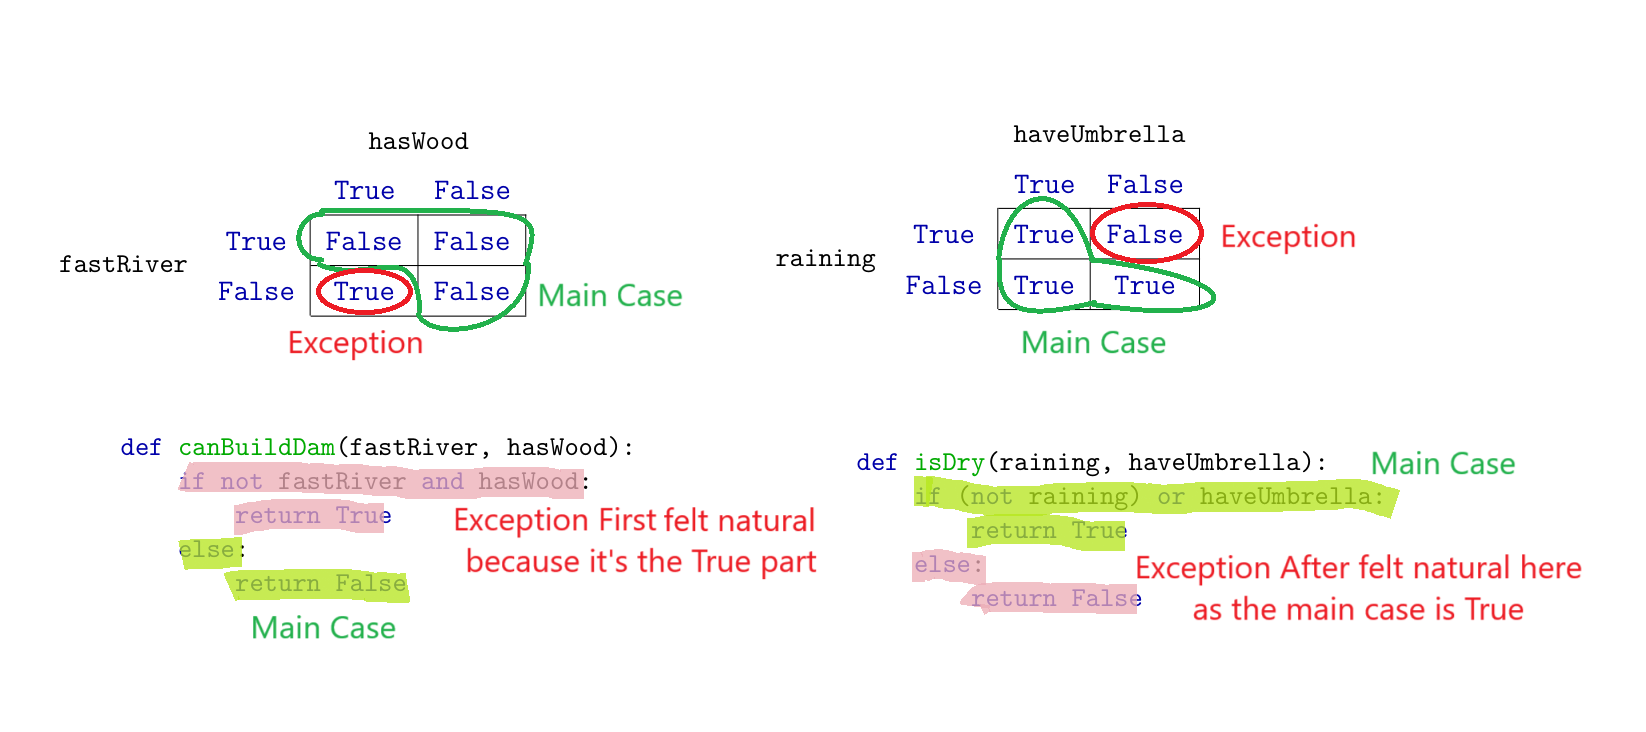
\includegraphics[scale=0.4]{Exception vs Main First.png}
    \caption*{The Thought Process in Coding}
\end{figure}

\newpage
\section{CodingBat Setup}
We'll be using CodingBat to develop your coding skills. It's a great website because it provides feedback instantly on whether your code works. But the website does look like it's from the 90's...

\begin{figure}[H]
    \centering
    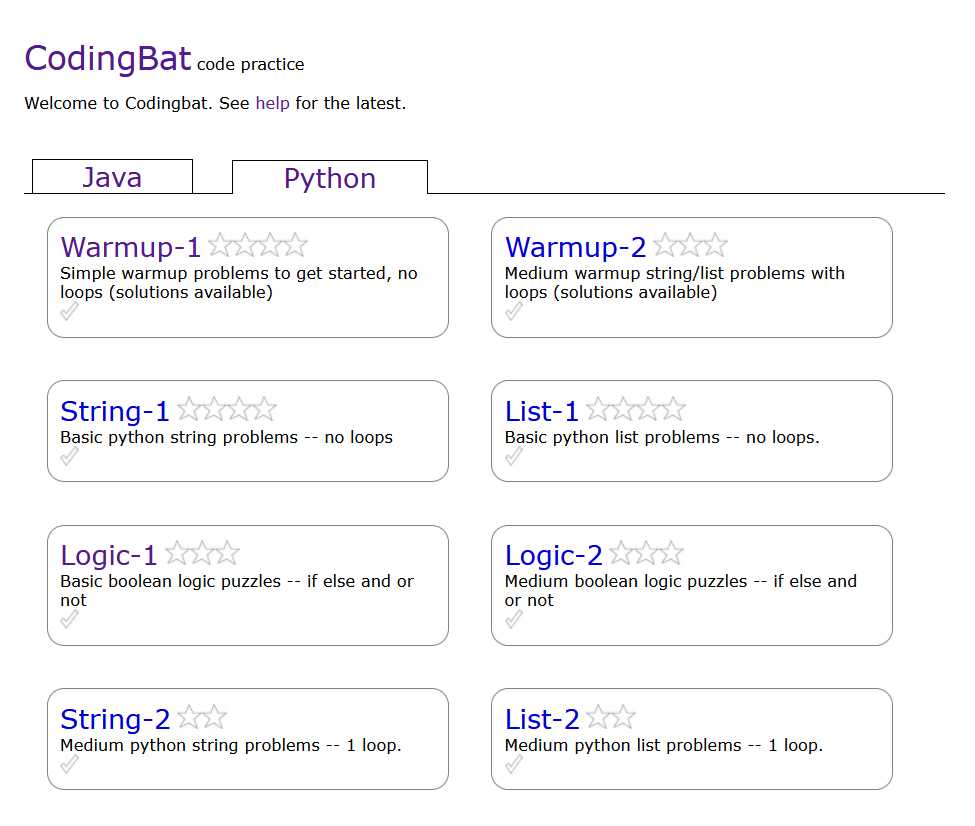
\includegraphics[scale=0.55]{CodingBat MainPage.png}
    \caption*{So retro!}
\end{figure}

\newpage
\hyperlink{https://codingbat.com/python}{Here's the link to the website.} In the top right corner, click the Create Account button to create your account.

\begin{figure}[H]
    \centering
    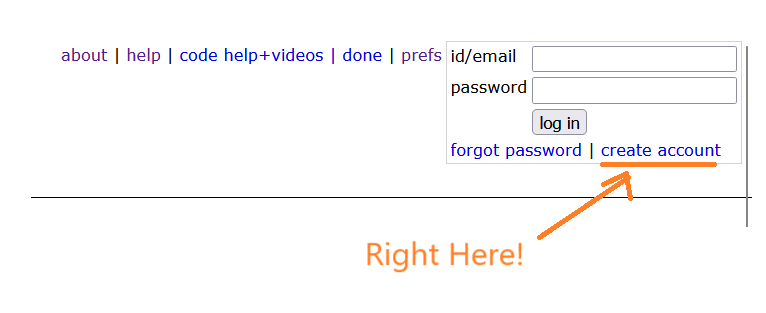
\includegraphics[scale=0.6]{CreateAccount.png}
    \caption*{Boom.}
\end{figure}

Do you see the \hyperlink{https://codingbat.com/pref}{prefs} link next to the login area in that image above? Click that after you create an account. This will let you add my email as an instructor so I can see your work. Make sure you click \underline{Share}.

\begin{figure}[H]
    \centering
    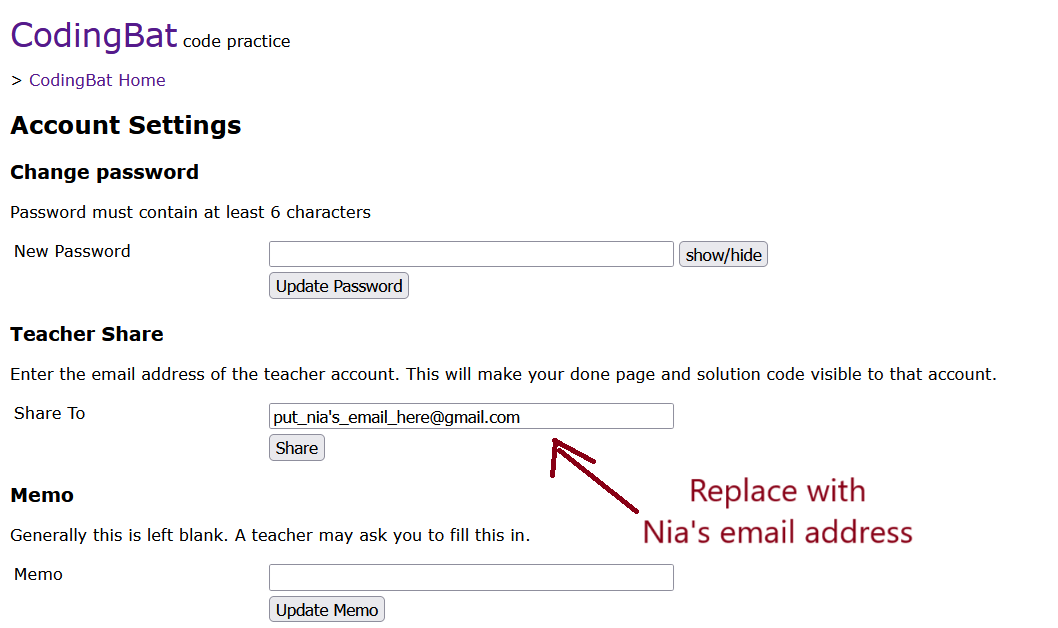
\includegraphics[scale=0.55]{TeacherShare.png}
    \caption*{And you're done!}
\end{figure}

From here, you can go back to the main page to access problems. It's coding time!

\section{Homework}
Some of the homework is CodingBat and some isn't. Have fun!
\begin{enumerate}
    \item Complete \codel{Warmup-1 $\to$ sleepIn}.
    \item Write the function for the following problem:
    \begin{callout}
        We can see stars if there are clear skies and there's no light pollution. Write a function \pythonl{canStargaze(cloudy, lightPollution)} that returns \pyTrue if we can see stars.
    \end{callout}
    Create a truth-table for the problem, a square, and write your solution in a \codel{.py} file. Then attempt to simplify your solution into one line if you feel confident enough.
    \item Complete \codel{Warmup-1 $\to$ monkeyTrouble}.
    \item Simplify the \pythonl{isDry} code into one-line:
    \begin{python}
        def isDry(raining, haveUmbrella):
            if (not raining) or haveUmbrella:
                return True
            else:
                return False
    \end{python}
    \item (Challenge) It's a 3 input problem!
    \begin{callout}
        A student is happy if there's no homework. But even if there's no homework, they're truly happy if the weather is nice or they have ice-cream. Write a function \pythonl{trulyHappy(haveHomework, niceWeather, haveIceCream)} that returns \pyTrue if the student is truly happy.
    \end{callout}
    We can't really use a square for this problem as we have 3 variables (try drawing a square to see what I mean). You would need a cube, and that's hard to draw. So I recommend creating a truth table instead with the following structure:
    \newcommand{\emptyboxed}{\boxed{\rule{0pt}{2ex}\qquad\qquad}}
    \begin{figure}[H]
        \centering
    \begin{tabular}{ccc|c}
        \pythonl{haveHomework} & \pythonl{niceWeather} & \pythonl{haveIceCream} & \pythonl{trulyHappy(|$\ldots$|)} \\
        \hline
        \pyFalse & \pyFalse & \pyFalse & \emptyboxed \\
        \pyFalse & \pyFalse & \pyTrue & \emptyboxed \\
        \pyFalse & \pyTrue & \pyFalse & \emptyboxed \\
        \pyFalse & \pyTrue & \pyTrue & \emptyboxed \\
        \pyTrue & \pyFalse & \pyFalse & \emptyboxed \\
        \pyTrue & \pyFalse & \pyTrue & \emptyboxed \\
        \pyTrue & \pyTrue & \pyFalse & \emptyboxed \\
        \pyTrue & \pyTrue & \pyTrue & \emptyboxed
    \end{tabular}
    \end{figure}

    This time we have 8 possibilities because 2 possibilites (True vs False) to the power of 3 inputs is $2^3 = 8$ possibilities. Fill in the boxes with whether the student is truly happy based on the problem description. You got this!
\end{enumerate}


\end{document}